% !TEX root = PREN2_Dokumentation.tex
\section{Realisierung}\label{realisierung}
\subsection{Initialisierungsphase}
\subsubsection{Kick-Off Meeting}
Das Kick-Off Meeting fand am 23.02.2021 als Zoom Meeting statt. Das Sitzungsprotokoll dazu ist im Kapitel \ref{kickOff} zu finden. \\
Es waren bei diesem Meeting alle Projektbeteiligten anwesend. In erster Linie wurde von Herr Meier das genaue Vorgehen bei der Bachelorarbeit vorgestellt. Anschliessend stellte der Auftraggeber das Projekt genauer vor und zeigte dabei seine Erwartungen auf. Die Aufgabenstellung wurde finalisiert und von allen Projektbeteiligten akzeptiert. Zudem schlug der Betreuer vor, im zwei bis drei Wochenrythmus ein Meeting abzuhalten. Im Anschluss wurde ein Termin für das erste Meeting vereinbart. 
\subsubsection{Erstellen des Projektmanagementplans}
Gemäss \ac{SoDa} wurde in einem ersten Projektschritt der Projektmanagementplan \ref{Projektmanagementplan}erstellt. In diesem wurde auch gleich der Rahmenplan erarbeitet. In diesem sind unter anderem die Meilensteine des Projekts dargestellt. Der Projektstrukturplan erleichterte dabei das Finden. Sie wurden in einem nächsten Schritt genauer spezifiziert und die Deliverables für ein erfolgreiches Erreichen des Meilensteins definiert. Durch den Projektstrukturplan konnten die einzelnen Teilbereiche des Projekts aufgelistet werden.
In der folgenden Risikoanalyse wurden die Risiken und entsprechenden Gegenmassnahmen erarbeitet. \\
Als letztes wurde die Projektunterstützung genauer spezifiziert. Dabei wurden die zu verwendenden Tools sowie die Elemente der Konfigurationseinheit festgelegt. \\
Als letzter Teil des Projektmanagements wurde die Teststrategie und die Testdrehbücher formuliert. Die Testdrehbücher werden während des Projekts vorlaufend formuliert. 

\subsubsection{Problem und Vision}
Das Kapitel \ref{Problem} wurde zum Beginn der Initialisierungsphase bearbeitet. Die Hauptprobleme konnten dabei sehr schnell gefunden werden. Die Vision des Projektes konnte mithilfe der Aussagen des Auftraggebers im Kick-Off Meeting \ref{kickOff} sehr gut beschrieben werden. 
\subsubsection{Requirement Engineering}
Beim Requirements Engineering diente die IEEE Spezifikation 29148-2018 als Grundlage [\cite{ieeeSrs}]. Um die Requirements zu finden, wurde in einem ersten Schritt eine Analyse der Aufgabenstellung durchgeführt. Ergänzt wurden diese durch Befragungen des Auftraggebers. Durch die so erlangten Informationen konnten die Anforderungen formuliert werden. In einem letzten Schritt wurden diese mit dem Auftraggeber besprochen. Hierbei wurden noch einige Anpassungen gemacht. 
\subsubsection{Stand der Technik}
In diesem Kapitel wurde eine Analyse der bestehenden, vergleichbaren Lösungen durchgeführt. Dabei wurde vorallem das Angebot der Post und von Valflora genauer betrachtet. Die bekannte \ac{PWA} von Starbucks zeigte dabei sehr gut deren Möglichkeiten auf. 
\subsubsection{Meilenstein Abschluss Initialisierungsphase}

\paragraph{Meilensteinbericht}
\subparagraph{Termin Meilenstein 2}
Der Meilenstein 2 ist am 07.03.2021 abgeschlossen und somit pünktlich fertiggestellt worden.
\subparagraph{Beschreibung Meilenstein 2}
Die Beschreibung des Meilensteins ist im Abschnitt \ref{Meilensteine} ersichtlich. 
\subparagraph{Meilensteinziele/Vorgaben}
Das übergeordnete Ziel dieses Meilensteins ist die Fertigstellung der Initialisierungsphase.
Hierzu war die Auslieferung der nachfolgenden Artefakte notwendig:
\begin{itemize}
	\item Projektmanagementplan
	\item Systemspezifikation
	\item Anforderungsliste
\end{itemize}
Zusätzlich wurden bereits die Kapitel \ref{Problem} und \ref{StandDerTechnik} fertiggestellt. 
\subparagraph{Meilensteinzielerreichung}
Es konnten alle geforderten Artefakte geliefert werden. Die Artefakte wurden bereits mit der Betreuungsperson im Meeting \ref{Beteuermeeting1} besprochen und konnten abgenommen werden. 
Der Meilenstein wurde erfolgreich erreicht. 
\subparagraph{Fazit}
Es wurden alle Artefakte erarbeitet. Der Meilenstein wurde somit erreicht und es kann weiter nach Plan gearbeitet werden.
\subsection{Konzeptionsphase}
\subsubsection{Sprint 1}\label{Sprint1}
\begin{table}[H]
	\begin{tabularx}{\textwidth}{|l|X|}
		\hline
		User Story & Number \\
		\hline
		Das System ist auf eine physische Pick-Up Station abgestimmt. & F.2\\
		\hline
	\end{tabularx} 
\caption[Userstories Sprint 1]{Userstories Sprint 1,\\ Quelle: Autor}
\end{table}\label{userStoriesSprint1}

\paragraph{Spezifikation der Schnittstelle zur Abholung}\label{SpezifikationSchnittstelleAbholung}
Um eine Abholung der Produkte zu bekommen, braucht es eine Kommunikation zwischen der \ac{PWA} und der Pick-Up Station. Um diese Schnittstelle genauer spezifizieren zu können, war es in einem ersten Schritt nötig, eine entsprechende Übertragungstechnologie festzulegen. Bei der Auswahl war dabei die Kompatibilität mit verschiedenen Geräten und Browsern ausschlaggebend. 
\subparagraph{NFC}
Als eine erste Idee wurde \ac{NFC} analysiert. \ac{NFC} eignet sich dabei ideal für die Übertragung von geringen Datenmenge. Dabei funktioniert es bis zu einer Distanz von 10cm. Die Umsetzung wäre dabei sehr einfach mittels einem Raspberry Pi umsetzbar. Einfache \ac{NFC}-Leser gibt es dabei schon für wenig Geld zu kaufen. Dabei könnte die gesamte Übertragung von der Informatik übernommen werden, eine weitere Schnittstelle zwischen Elektrotechnik und Informatik könnte dabei vermieden werden.  \\Die Technologie ist dabei sehr robust. Ein Überkleben oder Zerkratzen des Lesers hat keinen Einfluss auf die Funktionalität  [\cite{nfc}]. 
Der Abholvorgang wäre sehr einfach und schnell, da nur ein kurzer Kontakt mit dem Smartphone bereits ausreicht. 
\subparagraph{Kompatibilität}  
Apple schränkt den Zugriff von Webpages auf Standort-und Hardwaredienste unter iOS-Geräten sehr stark ein. Offiziell begründet wurde dies durch die Einschränkung von footprinting und des damit verbundenen Nutzertrackings. Für dieses Projekt ausschlaggebend ist dabei vor allem das Entfernen von NFC- und Bluetooth-Support. Somit ist es auch \ac{PWA}'s nicht mehr möglich, unter iOS auf die genannten Funktionen zuzugreifen [\cite{webKitTracking}].\\
Die Web-NFC-API wird zusätzlich bislang nur von Google Chrome unterstützt. Dies würde die Nutzbarkeit der Applikation sehr stark einschränken [\cite{kompWebNFC}]. 
Aus diesem Grund eignet sich \ac{NFC} nicht für die Verwendung in diesem Projekt. 
\subparagraph{QR-Code}\label{qrcode}
Die Restriktionen von Apple schränken die geeigneten Technologien sehr stark ein. Es bleibt nur noch der Zugriff auf die Kamera, um mit der Pick-Up Station zu kommunizieren. Ursprünglich war dies vom Auftraggeber nicht gewünscht. Das Verwenden einer anderen Technologie würde aber viel zu viele Einschränkungen führen, sodass die \ac{PWA} mit vielen Geräten unbrauchbar wäre. \\
Aus diesem Grund musste ein Konzept entwickelt werden, um die Warenausgabe mittels QR-Code auszulösen. Dabei sind zwei Ansätze möglich: 
\begin{itemize}
	\item Fixer QR-Code auf Pick-Up Station, wird von \ac{PWA} eingelesen. 
	\item Variabler QR-Code in \ac{PWA}, wird von Pick-Up Station eingelesen. 
\end{itemize}
Aus hardwaretechnischer Sicht ist die Umsetzung der ersten Lösung bedeutend einfacher Umzusetzen, bietet aber auch Fehlerpotential. Ein Überkleben des QR-Codes auf der Station würde die gesamte Station unbrauchbar machen. Eine Abholung der Bestellungen wäre nicht mehr möglich. \\
Die zweite Variante ist hardwaretechnisch anspruchsvoller. Auf der Pick-Up Station muss ein optischer Leser verbaut werden. Mit diesem kann der QR-Code aus der \ac{PWA} eingelesen und die Bestellung ausgegeben werden. \\

\begin{figure}[H]
	\centering
	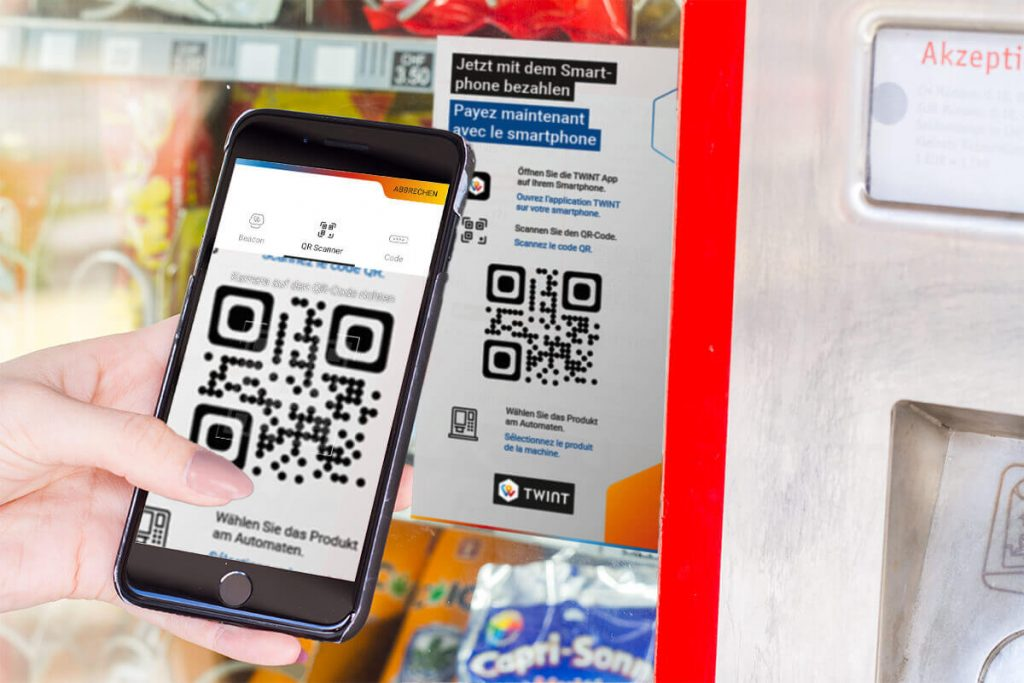
\includegraphics[width=1\textwidth]{images/QR-CodeOnMachine.jpg}
	\caption[Beispielanwendung QR-Code auf Gerät]{Beispielanwendung QR-Code auf Gerät,\\ Quelle: \cite{imageQRCodeTwint}}
	\label{img: Beispielanwendung QR-Code auf Geraet}
\end{figure}
Eine Grafik zum zweiten Lösungsansatz ist dabei im Kapitel \ref{avecBox} zu finden. 
Die genaue Wahl wird im Meeting mit dem Auftraggeber besprochen und abgesegnet. 

\subsubsection{Sprintreview Sprint 1}
Im Sprint 1 wurde eine genauere Analyse der Schnittstelle zur Produktabholung durchgeführt. Dabei müssen im Meeting von dieser Woche die gefundenen Lösungen mit dem Auftraggeber besprochen werden. Die Userstory kann erst zu Beginn des nächsten Sprints abgeschlossen werden. 

\paragraph{Meilensteinbericht}
\subparagraph{Termin Meilenstein 3}
Der Meilenstein 3 ist am 18.03.2021 abgeschlossen und somit mit drei Tagen Verspätung fertiggestellt worden. 
\subparagraph{Beschreibung Meilenstein 2}
Die Beschreibung des Meilensteins ist im Abschnitt \ref{Meilensteine} ersichtlich. 
\subparagraph{Meilensteinziele/Vorgaben}
Das übergeordnete Ziel dieses Meilensteins ist die Fertigstellung der Initialisierungsphase.
Hierzu war die Auslieferung der nachfolgenden Artefakte notwendig:
\begin{itemize}
	\item Projektmanagementplan
	\item Systemspezifikation
	\item Anforderungsliste
\end{itemize}
Zusätzlich wurden bereits die Kapitel \ref{Problem} und \ref{StandDerTechnik} fertiggestellt. 
\subparagraph{Meilensteinzielerreichung}
Es konnten alle geforderten Artefakte geliefert werden. Die Artefakte wurden bereits mit der Betreuungsperson im Meeting \ref{Beteuermeeting1} besprochen und konnten abgenommen werden. 
Der Meilenstein wurde erfolgreich erreicht. 
\subparagraph{Fazit}
Es wurden alle Artefakte erarbeitet. Der Meilenstein wurde somit erreicht und es kann weiter nach Plan gearbeitet werden.

\subsubsection{Sprint 2}
\begin{table}[H]
	\begin{tabularx}{\textwidth}{|l|X|}
		\hline
		\textbf{User Story} & \textbf{Number} \\
		\hline
		Das System ist auf eine physische Pick-Up Station abgestimmt. & F.2\\
		\hline
		Das System bietet dem Kunden die Möglichkeit, verschiedene Produkte zu bestellen. & F.6\\
		\hline
		Das System muss über eine CI/CD-Pipeline verfügen. & L.6 \\
		\hline
	\end{tabularx} 
	\caption[Userstories Sprint 2]{Userstories Sprint 2,\\ Quelle: Autor}
\end{table}\label{userStoriesSprint2}

\paragraph{CI/CD Pipeline}
Nach Absprache mit dem Auftraggeber im Meeting wurde entschieden, dass der Prototyp im EnterpriseLab laufen soll. Daraufhin wurde eine Maschine beantragt. Es handelt sich hierbei um ein Ubuntu 16.07 LTS. Die Applikationen sollen dabei als Docker Container deployed werden. \\
Zuerst wurde geplant, die Pipeline wie im offiziellen Tutorial des Enterpriselabs zu erstellen. Auf Anfrage wurde jedoch ein anderes Vorgehen empfohlen. Nachfolgend wird die Antwort zitiert.  \\\\
"Wenn es dein Ziel ist eine Spring Boot Applikation zu builden und dann auf der VM zu deployen dann würde den Container auf den Shared Runner unserer GitLab Instanz builden lassen und in die Container Registry deines Projekts pushen. Für die Deploy Stage der CI/CD Pipeline kannst du deine VM als privaten GitLab Runner registrieren und so ohne SSH login den Container von der Registry pullen und laufen lassen. Die SSL Termination mit Lets Encrypt würde ich mit einem separaten nginx Container lösen der reverse proxy spielt. Dieser kann dann einfach laufen und muss für Änderungen an der Spring Boot Applikation auch nie modifiziert werden.

Der Vorteil im Vergleich zur Docker Übung ist, dass hier alle Hosts von der GitLab CI/CD Pipeline kontrolliert werden. In der Übung ist der docker-cloud-exercise Host abgekapselt und pullt mit Watchtower einfach blind das neuste Image von einer Registry. Dieser Aufbau macht IMO mehr Sinn wenn man einfach Container Images von dritten konsumiert, aber ist weniger elegant wenn man selbst Kontrolle über die Source und CI/CD Pipelines hat." [\cite{emailEnterpriselab:private}]

In diesem Auszug aus der Email vom Enterpriselabmitarbeiter Cyrill von Uslar sind sehr viele Informationen enthalten. Es war ein mehrmaliges Durchlesen nötig, um sich darunter etwas vorstellen zu können. Anschliessend wurde die Pipelineerstellung in die wesentlichen Punkte aufgeteilt um umgesetzt.
\begin{itemize}
	\item Builden auf dem Shared Runner 
	\item Pushen in die Container Registry des Projekts
	\item VM als privaten Runner registrieren und deployen
	\item nginx server als reverse Proxy für SSL Termination
\end{itemize}

\subparagraph{Builden auf dem Shared Runner}
In diesem Projekt wird die Pipeline für zwei Projekte aufgesetzt. In einem ersten Schritt wurde dies nur für die Spring Applikation durchgeführt. 
Das Vorgehen unterscheidet sich dabei nur im Buildprozess. 
Um die Spring Applikation zu Builden, wurde das Dockerfile identisch zum Spring Boot Docker-Tutorial aufgebaut [\cite{springBootDocker}

\begin{verbatim}
FROM maven:3.6.3-jdk-11-slim
ARG JAR_FILE=target/*.jar
COPY ${JAR_FILE} app.jar
ENTRYPOINT ["java","-jar","/app.jar"]
\end{verbatim}
Entgegen dem Tutorial, in welchem noch die Java Version 11 genutzt wird, kommt hier direkt Java 16 zum Einsatz. \\\\
Anschliessend wurde das .gitlab-ci.yml File erstellt. Es wurde hier eine Anleitung aus dem Gitlab Blog genutzt. Diese ist jedoch nicht mehr ganz aktuell. Das Deployment wird hier zudem auf ein Kubernetes Cluster durchgeführt. Es musste daher individuell angepasst werden. Es konnte somit nur der Build-Teil übernommen werden. [\cite{springBootCI}]\\
Gitlab stellt zum Builden von Docker-Images bereits mehrere Shared-Runner zur Verfügung. 
\begin{figure}[H]
	\centering
	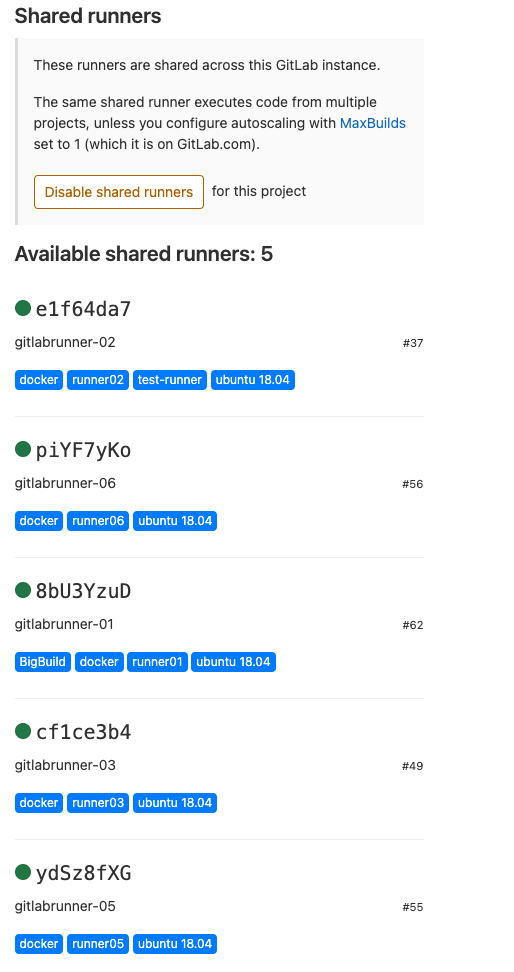
\includegraphics[scale=0.5]{images/gitLabRunner.png}
	\caption[Verfügbare Shared-Runner von GitLab]{Verfügbare Shared-Runner von GitLab,\\ Quelle: Autoren}
	\label{img: runnerGitlab}
\end{figure}
Der jeweilige Runner wird dabei mittels eines "fair usage algorithms" zugewiesen. Dabei ist die Anzahl der momentan auszuführenden Jobs pro Projekt entscheidend für die Wahl. Das Projekt mit den am wenigsten laufenden Jobs kommt zuerst. [\cite{runnersGitlab}] Zudem achtet der runner auf die verwendeten Tags. In diesem expliziten Beispiel sind mehrere Runner mit dem Docker-Tag versehen. Daher kann nicht sicher gesagt werden, welcher Runner den Docker Build durchführt. 
\subparagraph{Builden in die Registry des Projekt}
Um das erstellte Image in die Registry des Projekts zu pushen, werden von GitLab bereits die einzelnen Befehle vorgegeben. Diese können in die package-Stage integriert werden. 
\begin{figure}[H]
	\centering
	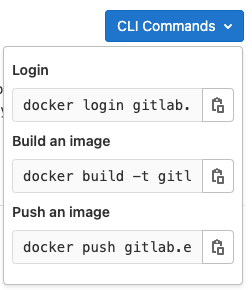
\includegraphics[scale=0.5]{images/gitLabRegistry.png}
	\caption[CLI Commands GitLab Container Registry]{CLI Commands GitLab Container Registry,\\ Quelle: Autoren}
\label{img: containerRegistryGitlab}
\end{figure}

Das entsprechende Image wird so in die interne Container Registry des GitLab Projekts gepushed. Dadurch kann auf das Verwenden eines Drittdienstes wie DockerHub verzichtet werden. 
Beim Build werden immer zwei Images in die Registry geschrieben. Einerseits eines mit dem Tag "latest" und eines mit dem Commit-Hash als Tag. Beim Deployment wird dann immer das Image mit dem aktuellen Commit-Hash verwendet. Dieser Mechanismus dient dazu, dass alle Versionen immer vorhanden sind. "Latest" zeigt dabei immer auf die aktuelle Version. 

\subparagraph{VM als privaten Runner registrieren und deployen}
Um das Deployment ohne Watchtower durchführen zu können, wurde auf die Virtuelle Maschine als Docker-Runner hinzugefügt. Es handelt sich somit dabei um einen specific Runner. 
GitLab Runner kann dabei einfach mittels Paketmanager auf Ubuntu installiert werden. Anschliessend musste dieser noch konfiguriert werden. Dazu musste der Token sowie die URL von GitLab dem Runner hinzugefügt. Der Runner ist anschliessend im Runner Bereich des Projekts zu finden. Zudem wurde anschliessend die Option "Lock to current projects" enfernt, sodass dieser Runner auch direkt für das Angular Projekt genutzt werden kann. 
Um ein SSH-Login zu vermeiden, wurde der Executor dabei als Shell-Executor definiert. Bei einem SSH-Executor wäre vorgängig die Verbindung via SSH nötig gewesen. 
Anschliessend können die entsprechenden Befehle für das Deployen in das gitlab-ci.yml integriert werden. Dabei war es zunächst ein Problem, dass die Berechtigung fehlte. Erst nach dem Login mittels GitLab CI-Token konnte der Container erfolgreich gepulled und anschliessend gestartet werden. 

\subparagraph{Build und Deployment des Frontends}
Um mit dem nächsten Schritt weiterzufahren, musste zuerst das Deployment des Angular Projekts konfiguriert werden. Hierbei liegt der Hauptunterschied in dem Build-Prozess. Dabei ist es wichtig, die beim Build entstehenden Artifakte in GitLab zu speichern. Nur so kann auf ein erneutes Builden beim Erstellen des Docker Containers verzichtet werden. Zudem werden die Node Module in den Cache gespeichert. Die nachfolgenden Befehle sind identisch zum Vorgehen bei Spring.  

\subparagraph{nginx als Reverse Proxy}
Um den nginx-Server gegen Zugriffe von Aussen zu schützen, wurde auf einen Reverse Proxy gesetzt. Der Reverse Proxy stellt dabei die einzige Verbindung ins öffentliche Netz dar. Zudem übernimmt er die Zertifikatsverwaltung des Frontends. Alternativ wäre auch ein Caching möglich, auf die Umsetzung wurde für diesen Anwendungsfall jedoch verzichtet. [\cite{reverseProxy}] \\\\

Die Umsetzung wurde dabei analog zum Tutorial von Alexander Bohndorf durchgeführt. [\cite{confReverseProxy}] Dabei wurde der nginx-proxy von jwilder sowie die damit kompatible letsencrypt companion verwendet. Die Umsetzung wurde dabei mittels docker-compose Files durchgeführt. 

\paragraph{Abschliessende Bemerkungen}
Das Erstellen der CI/CD Pipelines des Projekts verlief grösstenteils problemlos. Durch die Grundlage des Enterpriselabs und der sehr guten Dokumentation von GitLab konnte dies sehr schnell umgesetzt werden. Durch das Hinzufügen des Reverse Proxies konnte die Sicherheit des Systems massiv erhöht werden. Zusätzlich wurde so auch gleich die Auslieferung via HTTPS hinzugefügt sowie für ein immer gültiges Zertifikat gesorgt. \\
Beim Backend wurde auf eine zusätzliche Test-Stage verzichtet. Die gesamten Tests werden bereits im Maven-Build ausgeführt. Beim Frontendprojekt wurde dazu eine eigene Stage für e2e Tests festgelegt. 
Die fertigen Konfigurationen sind im GitLab Projekt enthalten und können dort eingesehen werden. 

\paragraph{Bestellen von Produkten}
Um eine Bestellung durchführen zu können, wurde in einem ersten Schritt das Article Object definiert. Basierend auf diesem wurde das passende \ac{DTO} definiert. Um das Mapping zwischen DTOs und Objekt zu vereinfachen, wurde der Object Mapper modelmapper genutzt. 
Zudem wurde direkt mit \ac{HATEOAS} gearbeitet. Der Controller stellt dabei die gewohnten CRUD-Operationen zur Verfügung. \\

\paragraph{Abstimmung auf physische Pick Up Station}
Im Meeting von dieser Woche wurden dem Auftraggeber die beiden in Kapitel \ref{qrcode} erarbeiteten Lösungen vorgestellt. Der Entscheid fiel dabei zugunsten der ersten Alternative. Dabei befindet sich der QR-Code fix auf der Station. Diese ist deutlich robuster und einfacher umzusetzen. \\\\
Die Schnittstellen zwischen Elektrotechnik und Informatik sind essentiell für die Funktionalität des Endprodukts. Aus diesem Grund wurde in diesem Sprint ein Meeting zwischen den Projektbeteiligten einberufen. Besonders das Senden der Ausgabeanforderung führte dabei zu Problemen. Hierbei soll auf einen Busy-Waiting Ansatz verzichtet werden. Jedoch soll die Lösung auch sehr energiesparend und effizient umsetzbar sein. Da beide Beteiligten keine Erfahrung im \ac{IoT}-Umfeld besitzen, wurde hier der Betreuer Michael Handschuh um Hilfe gebeten. 


\subsubsection{Sprintreview Sprint 2}
In Sprint 2 konnten nicht alle User Stories vollständig erfüllt werden. Es werden daher zwei von drei User Stories im nächsten Sprint weiter bearbeitet. Die Umsetzung der CI/CD Pipeline ist hingegen abgeschlossen. Dies war auch die Hauptarbeit in diesem Sprint. Für die Spezifizierung der Schnittstelle wird beim Meeting mit dem Betreuer eine geeignete Lösung erarbeitet. Bei dem Bestellprozess ist bereits die Abfrage von Produkten an der API möglich. In einem nächsten Schritt wird das passende Frontend entworfen und umgesetzt. 

\subsubsection{Sprint 3}
\paragraph{User Stories}
In diesem Sprint wurden keine neuen User Stories zum Sprint Backlog hinzugefügt. Es wird weiterhin an den beiden verbleibenden User Stories gearbeitet. 

\newpage
